\chapter{仿真实验与一致性测试}
\label{cha:evaluate}


\section{本章引言}
本章主要对RSCP-iBGP系统的功能进行了测试评价、对新系统下的新协议进行了一致性测试。功能验证方面,通过设计合理的网络拓扑,验证RSCP-iBGP系统,实现了路由存储和路由计算的集中优化、在路由计算的过程中基于全部路由且不存在因为MED不可比引起路由震荡等功能。本文提出的RSCP-iBGP新系统实际上对iBGP协议进行了改动,对RSCP-iBGP新系统下的新协议通过TTCN-3测试例进行一致性测试,很好地验证了RSCP-iBGP系统功能实现与设计的一致性。

\section{RSCP-iBGP系统功能验证实验}

第3章的例子都跑一遍,如何证明你的系统的正确性?
实验方面RCP和RFCP是怎么实现的?

\subsection{路由存储集中优化}

\subsection{路由计算集中优化}

\subsection{基于全部路由且无MED值引起的路由震荡}


\begin{figure}
  \centering
  % Requires \usepackage{graphicx}
  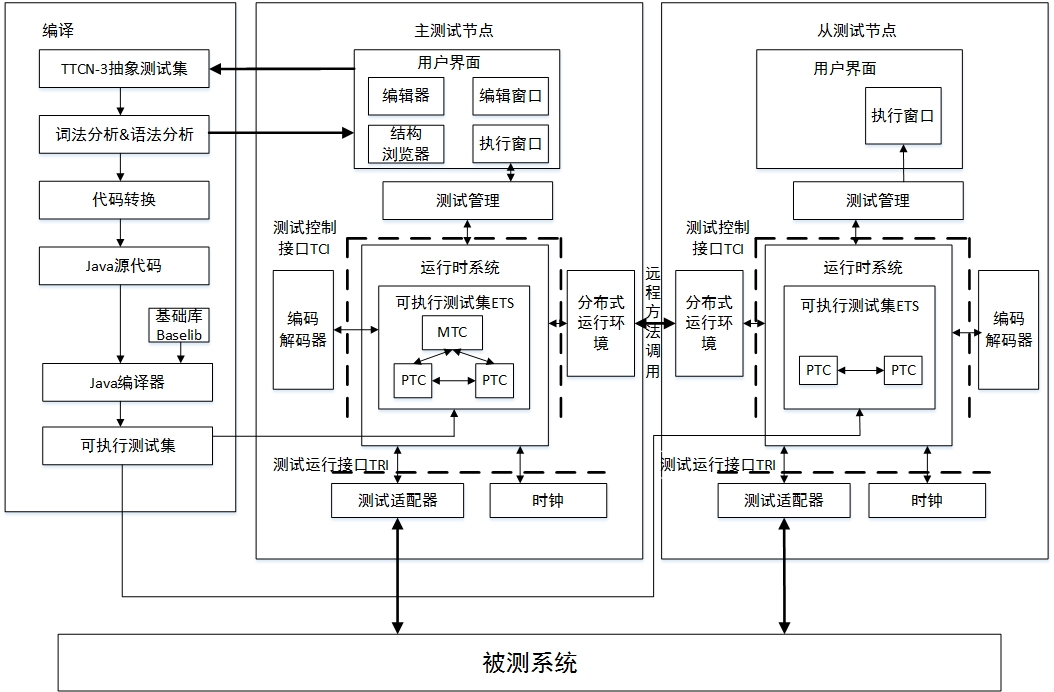
\includegraphics[width=0.75\textwidth]{pitsv3}
  \caption{PitSv3系统的体系结构\cite{pitsv3}}
  \label{fig:pitsv3}
\end{figure}


\section{协议的一致性测试}
\subsection{测试平台介绍}
测试平台使用协议测试系统工具PITSv3\cite{pitsv3}(Protocol Integrated Test System Version 3),PITSv3内通过主测试部件和多个从测试部件,来模拟测试系统多网口的情况,每个测试部件可以连接一个真实的虚拟路由器,以此来构建测试系统连接的网络拓扑,从而实现对协议的一致性测试。PITSv3系统的体系结构见图\ref{fig:pitsv3}。

本文中针对RSCP-iBGP系统的功能测试,依托安装在物理机器上的VMware Workstation Pro虚拟机管理软件,在VMware虚拟机管理软件中运行多台虚拟机,分别作为(安装PITSv3的Windows系统)测试系统和(运行RSCP-iBGP系统中的Route-Client软件路由器或者Route-Server软件路由器的CentOS系统)被测系统。

\subsection{一致性测试需求}

对RSCP-iBGP系统的测试主要分两个测试部分:对自治系统内的边界路由器Route-Client进行测试,对自治系统内的Route-Server进行测试,具体的测试需求如下。

% Please add the following required packages to your document preamble:
% \usepackage{multirow}
\begin{table}[]
\centering
\caption{RSCP-iBGP系统中Route-Client与eBGP邻居的一致性测试集}
\label{tab:test1}
\begin{tabular}{|c|c|l|}
\hline
测试组                                  & 测试用例     & 测试目的                                                                         \\ \hline
\multirow{4}{*}{Route-Client与eBGP邻居} & 邻居建连测试   & \begin{tabular}[c]{@{}l@{}}Route-Client可以接收\\ eBGP邻居的主动连接\end{tabular}       \\ \cline{2-3}
                                     & 对等体断连测试  & \begin{tabular}[c]{@{}l@{}}Route-Client可以处理\\ eBGP邻居的主动断连\end{tabular}       \\ \cline{2-3}
                                     & 前缀报文接收测试 & \begin{tabular}[c]{@{}l@{}}Route-Client可以收到\\ eBGP邻居的UPDATE报文\end{tabular}   \\ \cline{2-3}
                                     & 前缀报文处理测试 & \begin{tabular}[c]{@{}l@{}}Route-Client将eBGP邻居的路由更新\\ 附加Weight属性发给iBGP邻居\end{tabular} \\ \hline
\end{tabular}
\end{table}


被测系统Route-Client与eBGP邻居,进行eBGP邻居建连测试、eBGP对等体断连测试、eBGP对等体前缀报文接收测试、eBGP对等体前缀报文处理测试:
\begin{itemize}
  \item 被测系统Route-Client与eBGP邻居,进行eBGP邻居建连测试:测试系统软件向Route-Client被测系统发送OPEN报文,请求与Route-Client建立eBGP连接,当测试系统软件收到被测系统Route-Client回复过来的OPEN报文和KEEPALIVE报文,表明eBGP邻居建连成功;
  \item 被测系统Route-Client与eBGP邻居,进行eBGP对等体断连测试:测试系统软件向Route-Client被测系统发送OPEN报文,请求与Route-Client建立eBGP连接,当测试系统软件收到被测系统Route-Client回复过来的OPEN报文和KEEPALIVE报文,则邻居建连成功,测试系统回复KEEPALIVE报文维持连接,之后测试系统主动断开BGP连接,即连续三次收到Route-Client被测系统发来的KEEPALIVE不回复,最后测试系统收到了Route-Client被测系统通知断连的NOTIFICATION报文,表明eBGP对等体断连成功;
  \item 被测系统Route-Client与eBGP邻居,进行eBGP对等体前缀报文接收测试:测试系统软件和Route-Client被测系统建立eBGP连接,测试系统软件通过向Route-Client被测系统发送UPDATE报文信息,如果Route-Client被测系统正确接收到eBGP报文,Route-Client开启该eBGP对等体的Adj-RIB-In存储的情况下,能够查到收到的UPDATE报文信息,表明eBGP对等体前缀报文接收成功;
  \item 被测系统Route-Client与eBGP邻居,进行eBGP对等体前缀报文处理测试:测试系统软件端口A和Route-Client被测系统建立eBGP连接,测试系统软件端口B和Route-Client被测系统建立iBGP连接。测试系统软件端口A通过向Route-Client被测系统发送UPDATE报文信息,如果Route-Client被测系统正确接收到eBGP报文,Route-Client开启该eBGP对等体的Adj-RIB-In存储的情况下,能够查到收到的UPDATE报文信息,表明eBGP对等体前缀报文接收成功;此时测试系统端口B收到了Route-Client发过来的携带Weight属性信息的UPDATE报文(配置Route-Client被测系统从某eBGP对等体收到路由的Weight值),表明eBGP对等体前缀报文处理正确。\\
\end{itemize}


\begin{table}[]
\centering
\caption{RSCP-iBGP系统中Route-Client与iBGP邻居的一致性测试集}
\label{tab:test2}
\begin{tabular}{|c|c|l|}
\hline
测试组                                  & 测试用例     & 测试目的                                                                         \\ \hline
\multirow{4}{*}{Route-Client与iBGP邻居} & 邻居建连测试   & \begin{tabular}[c]{@{}l@{}}Route-Client可以接收\\ iBGP邻居的主动连接\end{tabular}       \\ \cline{2-3}
                                     & 对等体断连测试  & \begin{tabular}[c]{@{}l@{}}Route-Client可以处理\\ iBGP邻居的主动断连\end{tabular}       \\ \cline{2-3}
                                     & 前缀报文接收测试 & \begin{tabular}[c]{@{}l@{}}Route-Client可以收到\\ iBGP邻居的UPDATE报文\end{tabular}   \\ \cline{2-3}
                                     & 前缀报文处理测试 & \begin{tabular}[c]{@{}l@{}}Route-Client可将iBGP邻居\\ 的路由更新宣告给所有eBGP邻居\end{tabular} \\ \hline
\end{tabular}
\end{table}


被测系统Route-Client与iBGP邻居,进行iBGP邻居建连测试、iBGP对等体断连测试、iBGP对等体前缀报文接收测试、iBGP对等体前缀报文处理测试:
\begin{itemize}
  \item 被测系统Route-Client与iBGP邻居,进行iBGP邻居建连测试:测试系统软件向Route-Client被测系统发送OPEN报文,请求与Route-Client建立iBGP连接,当测试系统软件收到被测系统Route-Client回复过来的OPEN报文和KEEPALIVE报文,表明iBGP邻居建连成功;
  \item 被测系统Route-Client与iBGP邻居,进行iBGP对等体断连测试:测试系统软件向Route-Client被测系统发送OPEN报文,请求与Route-Client建立iBGP连接,当测试系统软件收到被测系统Route-Client回复过来的OPEN报文和KEEPALIVE报文,则邻居建连成功,测试系统回复KEEPALIVE报文维持连接,之后测试系统主动断开BGP连接,即连续三次收到Route-Client被测系统发来的KEEPALIVE不回复,最后测试系统收到了Route-Client被测系统通知断连的NOTIFICATION报文,表明iBGP对等体断连成功;
  \item 被测系统Route-Client与iBGP邻居,进行iBGP对等体前缀报文接收测试:测试系统软件和Route-Client被测系统建立iBGP连接,测试系统软件通过向Route-Client被测系统发送UPDATE报文信息,如果Route-Client被测系统正确接收到iBGP报文,Route-Client开启该iBGP对等体的Adj-RIB-In存储的情况下,能够查到收到的UPDATE报文信息,表明iBGP对等体前缀报文接收成功;
  \item 被测系统Route-Client与iBGP邻居,进行iBGP对等体前缀报文处理测试:测试系统软件端口A和Route-Client被测系统建立eBGP连接,测试系统软件端口B和Route-Client被测系统建立eBGP连接,测试系统软件端口C和Route-Client被测系统建立iBGP连接。测试系统软件端口C通过向Route-Client被测系统发送UPDATE报文信息,如果Route-Client被测系统正确接收到iBGP报文,Route-Client开启该iBGP对等体的Adj-RIB-In存储的情况下,能够查到收到的UPDATE报文信息,表明iBGP对等体前缀报文接收成功;此时测试系统端口A和B收到了Route-Client转发过来的从iBGP收到的前缀的最优路由的UPDATE报文,表明iBGP对等体前缀报文,表明iBGP对等体前缀报文处理正确。\\
\end{itemize}





\begin{table}[]
\centering
\caption{RSCP-iBGP系统中Route-Server与iBGP邻居的一致性测试集}
\label{tab:test3}
\begin{tabular}{|c|c|l|}
\hline
测试组                                  & 测试用例     & 测试目的                                                                         \\ \hline
\multirow{4}{*}{\begin{tabular}[c]{@{}c@{}}Route-Server与\\ iBGP邻居\end{tabular}} & 邻居建连测试   & \begin{tabular}[c]{@{}l@{}}Route-Server可以接收\\ iBGP邻居的主动连接\end{tabular}       \\ \cline{2-3}
                                     & 对等体断连测试  & \begin{tabular}[c]{@{}l@{}}Route-Server可以处理\\ iBGP邻居的主动断连\end{tabular}       \\ \cline{2-3}
                                     & 前缀报文接收测试 & \begin{tabular}[c]{@{}l@{}}Route-Server可以收到iBGP邻居\\ 的带Weight属性值的UPDATE报文\end{tabular}   \\ \cline{2-3}
                                     & 前缀报文处理测试 & \begin{tabular}[c]{@{}l@{}}Route-Server收到iBGP邻居的路由更新,计算\\ iBGP邻居对应最优路由并宣告给每个iBGP邻居\end{tabular} \\ \hline
\end{tabular}
\end{table}


被测系统Route-Server与iBGP邻居,进行iBGP邻居建连测试、iBGP对等体断连测试、iBGP对等体前缀报文接收测试、iBGP对等体前缀报文处理测试:
\begin{itemize}
  \item 被测系统Route-Server与iBGP邻居,进行iBGP邻居建连测试:测试系统软件向Route-Server被测系统发送OPEN报文,请求与Route-Server建立iBGP连接,当测试系统软件收到被测系统Route-Server回复过来的OPEN报文和KEEPALIVE报文,表明iBGP邻居建连成功;
  \item 被测系统Route-Server与iBGP邻居,进行iBGP对等体断连测试:测试系统软件向Route-Server被测系统发送OPEN报文,请求与Route-Server建立iBGP连接,当测试系统软件收到被测系统Route-Server回复过来的OPEN报文和KEEPALIVE报文,则邻居建连成功,测试系统回复KEEPALIVE报文维持连接,之后测试系统主动断开BGP连接,即连续三次收到Route-Server被测系统发来的KEEPALIVE不回复,最后测试系统收到了Route-Server被测系统通知断连的NOTIFICATION报文,表明iBGP对等体断连成功;
  \item 被测系统Route-Server与iBGP邻居,进行iBGP对等体前缀报文接收测试:测试系统软件和Route-Server被测系统建立iBGP连接,测试系统软件通过向Route-Server被测系统发送UPDATE报文信息,如果Route-Server被测系统正确接收到携带Weight属性信息的UPDATE报文,表明iBGP对等体前缀报文接收成功;
  \item 被测系统Route-Server与iBGP邻居,进行iBGP对等体前缀报文处理测试:测试系统软件端口A和Route-Server被测系统建立iBGP连接,测试系统软件端口B和Route-Server被测系统建立iBGP连接,测试系统软件端口C和Route-Server被测系统建立iBGP连接。测试系统软件端口A通过向Route-Server被测系统发送2条相同前缀不同路由的UPDATE报文信息,如果Route-Server被测系统正确接收到该2条路由信息,表明iBGP对等体前缀报文接收成功;此时测试系统端口A、B和C收到了Route-Server被测系统发来的该前缀的最优路由的UPDATE报文,表明被测系统Route-Server与iBGP对等体之间的前缀报文处理正确。
\end{itemize}



\subsection{测试集设计}

本文提出的RSCP-iBGP系统在自治系统内部有两种类型的路由器Route-Client边界路由器和Route-Server路由集中控制平台上的,Route-Client路由器有eBGP对等体和iBGP对等体,而Route-Server路由器仅有iBGP对等体。根据测试需求设计三组测试集共3个:Route-Client与eBGP邻居之间的一致性测试集如表\ref{tab:test1}、Route-Client与iBGP邻居之间的一致性测试集如表\ref{tab:test2}、Route-Server与iBGP邻居之间的一致性测试集如表\ref{tab:test3}。


\subsection{测试结果及分析}

针对以上的测试需求和测试方案,本文对所有测试集中的测试例共12个进行测试,测试结果如表\ref{tab:res},从表中我们可以看出测试例全部通过,证明RSCP-iBGP系统实现与设计规范的一致性。



\section{本章小结}

本章主要对RSCP-iBGP系统的进行了功能验证、BGP扩展协议一致性测试。通过本章的仿真实验和协议测试,本文实现的RSCP-iBGP系统在性能实现上达到了最初的设计目标:基于全部路由进行路由计算,集合缩小式的新型路由算法也能避免MED不可比引起的路由震荡,路由表在集中平台上存储优化。在本文提出的RSCP-iBGP系统中,自治系统内部的路由计算次数和路由存储大小均优化了一个数量级,且不存在路由震荡和路由收敛等情况。
% Please add the following required packages to your document preamble:
% \usepackage{booktabs}
\begin{table}[]
\centering
\caption{RSCP-iBGP系统一致性测试集的测试结果}
\label{tab:res}
\begin{tabular}{@{}ccc@{}}
\toprule
测试集名称               & 通过用例数 & 失败用例数 \\ \midrule
Route-Client与eBGP邻居 & 4     & 0     \\
Route-Client与iBGP邻居 & 4     & 0     \\
Route-Server与iBGP邻居 & 4     & 0     \\
总计                  & 12    & 0     \\ \bottomrule
\end{tabular}
\end{table}